%%%%%%%%%%%%%%%%%% Preamble
\documentclass[12pt, letterpaper]{article}
\usepackage[utf8]{inputenc}
\usepackage{graphicx} % For Pictures
\usepackage{hyperref} % Links
% Link Color Setup
\hypersetup{
    pdftitle={LaTeX Tutorial},
    colorlinks=true,
    linkcolor=blue
    }

\graphicspath{ {../image} } % Set Image folder paths

\title{My Tutorial of \LaTeX \thanks{Learned from the Overleaf team}}
\author{Kittipos Sirivongrungson }
\date{January 2021}

%%%%%%%%%%%%%%%%%% Body
\begin{document}

% Add `title` `author` `date` to the docs 
\maketitle

% Abstract
\begin{abstract}
    
    This is a simple tutorial example from \href{https://github.com/Lightbridge-KS/LaTeX-tutorial}{my github repo}.
    Enjoy the show!

\end{abstract}

\tableofcontents % Cool TOC

\newpage

% Paragraph
\section{Paragraph}
Now that we have written our abstract, we can begin writing our first paragraph.
 
This line will start a second Paragraph.


% Text formatting
\section{Text Formatting}

\paragraph{Output:}
\textbf{Bold} \textit{Italics} \emph{Emphasized} \texttt{code}

Some of the \textbf{greatest} discovery in the \textit{science} were made by \textbf{\textit{accident}}


% List
\section{List}
%% Unordered List
\subsection{Unordered List}
\begin{itemize}
    \item Fruit
    \item Vegetable
\end{itemize}

%% Ordered List
\subsection{Ordered List}
\begin{enumerate}
    \item One
    \item Two
\end{enumerate}

\section{Math Stuff}

\section{Links}
It's also possible to link directly any word 
or \hyperlink{thesentence}{any sentence} in you document.

If you read this text, you will get no information.  Really?  
Is there no information?

For instance \hypertarget{thesentence}{this sentence}.

\subsection{Inline Mode}
The mass-energy equivalence is stated by the equation $E=mc^2$.

\subsection{Display Mode}
The mass-energy equivalence is described by the famous equation
\[ E=mc^2 \]
discovered in 1905 by Albert Einstein. 

% Graphic
\section{Graphic}
\subsection{Simple Figure}

\includegraphics[scale = 0.2]{octocat.png} % File extension is advised not to include, but I will.

% Graphic with Caption & Labels
\subsection{Figure with Caption and Labels}
\begin{figure}[h]
    \centering
    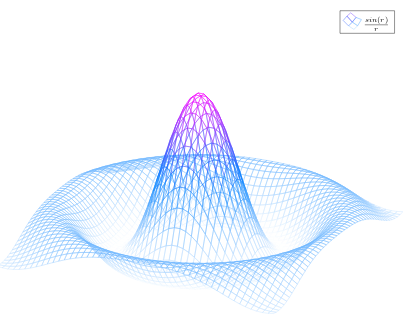
\includegraphics[scale = 0.5]{mesh}
    \caption{a nice plot}
    \label{fig:mesh1}
\end{figure}

As you can see in the figure \ref{fig:mesh1}, the function grows near 0. Also, in the page \pageref{fig:mesh1} 
is the same example.

\section{Tables}   

\begin{center}
    \begin{tabular}{c c c}
        cell1 & cell2 & cell3 \\ 
        cell4 & cell5 & cell6 \\  
        cell7 & cell8 & cell9 
    \end{tabular}
\end{center}


\end{document}